% This is the section of the results focused on the assembly


\section{Transcriptome Assembly}

\subsection{Assembly Quality}
\subsubsection{Quality Statistics}
\subsubsection{Example Transcripts}
To assess the data/assembly quality further, I used canonical transcripts of \textit{C. acetobutylicum} for comparison. Six issues, listed below, were considered for each example to better understand the quality of the assembly and the degree of curation required. 
\begin{enumerate}
\item Is the transcript large enough to include the known ORFs and RBSes?
\item Does the assembled transcript's TSS agree with promoter motifs?
\item Does it agree with published transcription start sites?
\item Does the assembled transcript's size agree with published Northern blots?
\item Does the assembly represent the coverage and if not, which best represents the biological knowledge of this region?
\item Does the assembled region require curation (e.g. fused or truncated transcripts)?
\end{enumerate}
Agreement between the data and the literature would support the efficacy of this technique. Furthermore, these results could be widely applicable to future studies if only minimal curation is required. The first example that I examine is the Sol locus.

The Sol locus is a 5.1kb region(175530-180,650) on the pSol1 megaplasmid that is responsible for the production of several solvents. This region encodes several enzymes including a tri-functional NAD(H\textsuperscript{+})-dependent alcohol/aldehyde dehydrogenase, two coenzyme-A transferases, and a acetoacetate decarboxylase. These genes are vital for acid reuptake and conversion into alcohols, a vital part of this organism's metabolism.
In this dataset, we observe strong coverage (> 10,000x) of the Sol operon and ADC. The Sol operon has continuous coverage across the entire 4.1kb transcript and its size agrees with the literature. The regulatory protein SolR has a lower degree of coverage (> 300x), yet its 1.1kb size is corroborated by additional studies.
The assembly suggests a distal transcription start site for the Sol operon at 175,564, agreeing with two previous studies of this region. Several increases in coverage are observed just after the proximal promoter as well. It is understood that the proximal promoter is the most active promoter motif for the Sol operon and this view is supported by our data. The assembly also shows a distinct transcription start site for SolR, in agreement with previous findings. The coverage data also agree with the single transcription start site for Adc, shown as a distinct increase in coverage. However, the Adc transcript has been misassembled, fused to residual signal upstream of the true TSS. This is the first example of misassembly, which I address in the next section.
The depth of coverage is also fairly consistent across these regions, except for a ~100bp region near the N-terminus of CtfA. This decrease in coverage can be explained by an inverted repeat present in this region, which could be difficult to sequence. It is also interesting to note that a promoter motif TTCATA(13)TATAAT is also present in the region, upstream of the RBS. Primer extension studies for this operon frequently use probes from AdhE, at the exclusion of CtfA. Additionally, most Northern blot analyses of this region follow the work of Durre et al, where probes were only designed for AdhE. In one source, a faint band is visible for a ~2.6kb RNA, which matches reasonably to the 2.7kb continuous sequence that we observe for AdhE in this example. Unfortunately, many other studies of this locus use AdhE probes exclusively and/or have sliced or semi-quantified their blots for publication, preventing further investigation of alternate bands.



%      Figure '1' Sol Locus
\begin{figure}
\small
{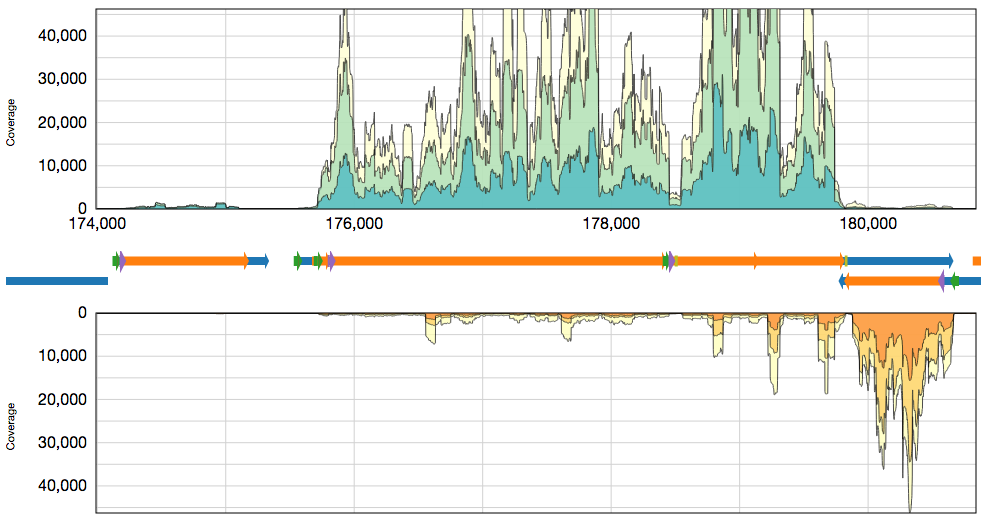
\includegraphics[width=\textwidth,height=2.5in]{images/Assembly/Sol/Sol-locus.png}
\subcaption{Sol locus}\label{fig:1a}}


% \label{fig:1}
\caption{Sol Locus: The Sol operon (\subref{fig:1a}) upper track) consists of OrfL, alcohol dehydrogenase (AdhE), and Co-A transferases A and B (ctfA,ctfB). Acetoacetate decarboxylase (ADC; \subref{fig:1a} lower track, right) is also shown. Coverage for the Watson and Crick strands (top and bottom tracks) are visualized with an annotation track (center). Tracks show cumulative coverage for unstressed (yellow), butanol (light green/ light orange), and butyrate (green/orange) stressed samples over all time points. Transcripts (blue), ORFs (orange), RBSes (purple), inverted repeats (yellow), promoters (green), and TSSes (red) are represented as arrows and bars.}
\end{figure}
\begin{figure}
\small
{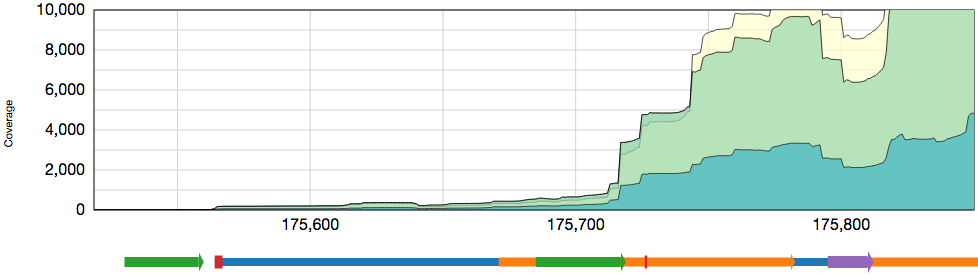
\includegraphics[width=\textwidth,height=1.5in]{images/Assembly/Sol/Sol-TSS.png}
\subcaption{Sol operon transcription initiation region}\label{fig:2a}}
{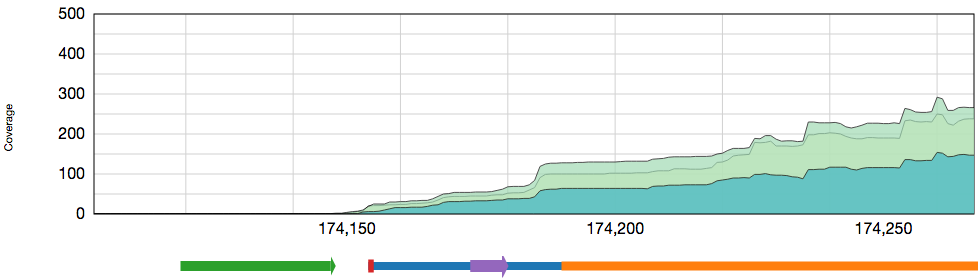
\includegraphics[width=\textwidth,height=1.5in]{images/Assembly/Sol/Sol-SolR-TSS.png}
\subcaption{SolR transcription initiation region}\label{fig:2b}}
{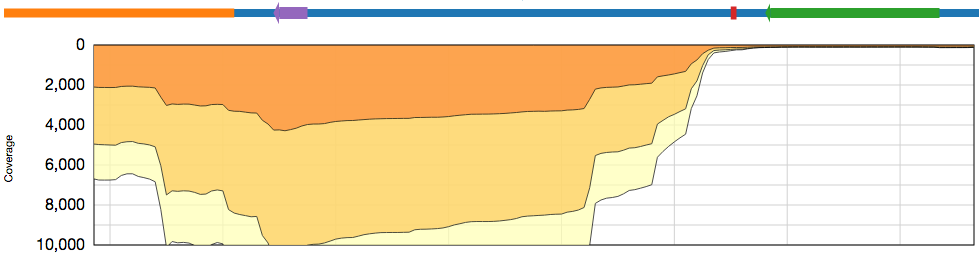
\includegraphics[width=\textwidth,height=1.5in]{images/Assembly/Sol/Sol-Adc-TSS.png}
\subcaption{Adc transcription initiation region}\label{fig:2c}}
%\label{fig:1.5}
\caption{Sol Locus Transcription Start Sites: . \subref{fig:2a}) Sol operon (OrfL, AdhE) transcription start sites. The coverage and assembly data have strong agreement with previously described proximal and distal promoters and transcription start sites. \subref{fig:2b}) The assembled transcription start site for SolR agrees with previous findings. \subref{fig:2b}) Transcription initiation region for Adc. While the coverage clearly shows the appropriate increase, the transcription start site has been fused to residual coverage upstream of the true TSS. }
\end{figure}
\begin{figure}
{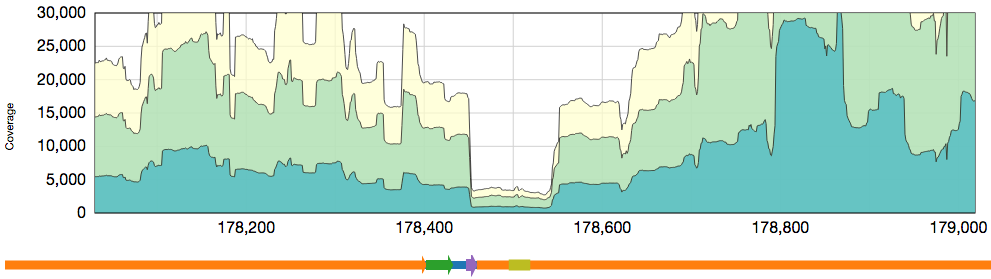
\includegraphics[width=\textwidth,height=1.5in]{images/Assembly/Sol/Sol-AdhE-terminator.png}
\subcaption{Putative AdhE terminator, CtfA/B promoter}\label{fig:3a}}
{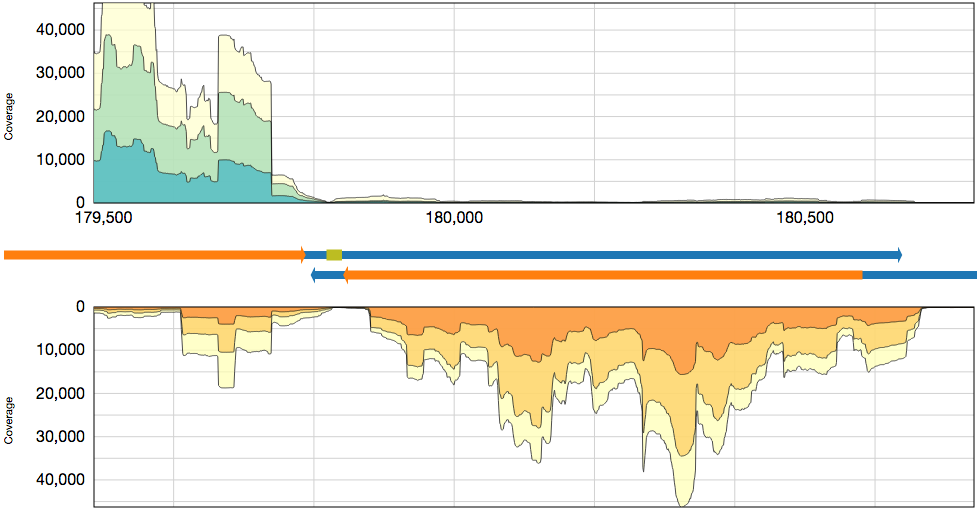
\includegraphics[width=\textwidth,height=2.5in]{images/Assembly/Sol/Sol-bifunctional-terminator}
\subcaption{Bifunctional Rho-independent terminator for Sol operon, Adc}\label{fig:3b}}
\caption{Sol Locus Transcription Stop Sites: \subref{fig:3a}) Low coverage in the Sol operon. A terminator may be partially responsible for a sustained low coverage level in the Sol operon. Additionally, a promoter motif was located upstream of the CtfA RBS and the pattern of expression is consistent with the beginning of a new transcript. \subref{fig:3b}) A bifunctional terminator, likely responsible for the decrease in coverage observed for both transcripts on their respsective strands}
\end{figure}

The next example that I consider involves BdhA and BdhB.


\subsection{Identify and Attempt to Resolve Remaining Issues}

\subsection{Novel Transcripts}

\subsection{Exploratory Tools}


